% Options for packages loaded elsewhere
\PassOptionsToPackage{unicode}{hyperref}
\PassOptionsToPackage{hyphens}{url}
%
\documentclass[
  ignorenonframetext,
  aspectratio=169,
]{beamer}
\usepackage{pgfpages}
\setbeamertemplate{caption}[numbered]
\setbeamertemplate{caption label separator}{: }
\setbeamercolor{caption name}{fg=normal text.fg}
\beamertemplatenavigationsymbolsempty
% Prevent slide breaks in the middle of a paragraph
\widowpenalties 1 10000
\raggedbottom
\setbeamertemplate{part page}{
  \centering
  \begin{beamercolorbox}[sep=16pt,center]{part title}
    \usebeamerfont{part title}\insertpart\par
  \end{beamercolorbox}
}
\setbeamertemplate{section page}{
  \centering
  \begin{beamercolorbox}[sep=12pt,center]{part title}
    \usebeamerfont{section title}\insertsection\par
  \end{beamercolorbox}
}
\setbeamertemplate{subsection page}{
  \centering
  \begin{beamercolorbox}[sep=8pt,center]{part title}
    \usebeamerfont{subsection title}\insertsubsection\par
  \end{beamercolorbox}
}
\AtBeginPart{
  \frame{\partpage}
}
\AtBeginSection{
  \ifbibliography
  \else
    \frame{\sectionpage}
  \fi
}
\AtBeginSubsection{
  \frame{\subsectionpage}
}

\usepackage{amsmath,amssymb}
\usepackage{iftex}
\ifPDFTeX
  \usepackage[T1]{fontenc}
  \usepackage[utf8]{inputenc}
  \usepackage{textcomp} % provide euro and other symbols
\else % if luatex or xetex
  \usepackage{unicode-math}
  \defaultfontfeatures{Scale=MatchLowercase}
  \defaultfontfeatures[\rmfamily]{Ligatures=TeX,Scale=1}
\fi
\usepackage{lmodern}
\usecolortheme{whale}
\ifPDFTeX\else  
    % xetex/luatex font selection
\fi
% Use upquote if available, for straight quotes in verbatim environments
\IfFileExists{upquote.sty}{\usepackage{upquote}}{}
\IfFileExists{microtype.sty}{% use microtype if available
  \usepackage[]{microtype}
  \UseMicrotypeSet[protrusion]{basicmath} % disable protrusion for tt fonts
}{}
\makeatletter
\@ifundefined{KOMAClassName}{% if non-KOMA class
  \IfFileExists{parskip.sty}{%
    \usepackage{parskip}
  }{% else
    \setlength{\parindent}{0pt}
    \setlength{\parskip}{6pt plus 2pt minus 1pt}}
}{% if KOMA class
  \KOMAoptions{parskip=half}}
\makeatother
\usepackage{xcolor}
\newif\ifbibliography
\setlength{\emergencystretch}{3em} % prevent overfull lines
\setcounter{secnumdepth}{-\maxdimen} % remove section numbering


\providecommand{\tightlist}{%
  \setlength{\itemsep}{0pt}\setlength{\parskip}{0pt}}\usepackage{longtable,booktabs,array}
\usepackage{calc} % for calculating minipage widths
\usepackage{caption}
% Make caption package work with longtable
\makeatletter
\def\fnum@table{\tablename~\thetable}
\makeatother
\usepackage{graphicx}
\makeatletter
\def\maxwidth{\ifdim\Gin@nat@width>\linewidth\linewidth\else\Gin@nat@width\fi}
\def\maxheight{\ifdim\Gin@nat@height>\textheight\textheight\else\Gin@nat@height\fi}
\makeatother
% Scale images if necessary, so that they will not overflow the page
% margins by default, and it is still possible to overwrite the defaults
% using explicit options in \includegraphics[width, height, ...]{}
\setkeys{Gin}{width=\maxwidth,height=\maxheight,keepaspectratio}
% Set default figure placement to htbp
\makeatletter
\def\fps@figure{htbp}
\makeatother

\setbeamertemplate{navigation symbols}{} 
\setbeamertemplate{footline}[page number]
\titlegraphic{
  
\includegraphics[width=2cm]{style/UZH.jpg}
  \hspace*{2cm}~%
  
\includegraphics[width=2cm]{style/FHNW.png}
  \hspace*{2cm}~%
  
\includegraphics[width=1cm]{style/BFH.png}
  }
\makeatletter
\makeatother
\makeatletter
\makeatother
\makeatletter
\@ifpackageloaded{caption}{}{\usepackage{caption}}
\AtBeginDocument{%
\ifdefined\contentsname
  \renewcommand*\contentsname{Table of contents}
\else
  \newcommand\contentsname{Table of contents}
\fi
\ifdefined\listfigurename
  \renewcommand*\listfigurename{List of Figures}
\else
  \newcommand\listfigurename{List of Figures}
\fi
\ifdefined\listtablename
  \renewcommand*\listtablename{List of Tables}
\else
  \newcommand\listtablename{List of Tables}
\fi
\ifdefined\figurename
  \renewcommand*\figurename{Figure}
\else
  \newcommand\figurename{Figure}
\fi
\ifdefined\tablename
  \renewcommand*\tablename{Table}
\else
  \newcommand\tablename{Table}
\fi
}
\@ifpackageloaded{float}{}{\usepackage{float}}
\floatstyle{ruled}
\@ifundefined{c@chapter}{\newfloat{codelisting}{h}{lop}}{\newfloat{codelisting}{h}{lop}[chapter]}
\floatname{codelisting}{Listing}
\newcommand*\listoflistings{\listof{codelisting}{List of Listings}}
\makeatother
\makeatletter
\@ifpackageloaded{caption}{}{\usepackage{caption}}
\@ifpackageloaded{subcaption}{}{\usepackage{subcaption}}
\makeatother
\makeatletter
\@ifpackageloaded{tcolorbox}{}{\usepackage[skins,breakable]{tcolorbox}}
\makeatother
\makeatletter
\@ifundefined{shadecolor}{\definecolor{shadecolor}{rgb}{.97, .97, .97}}
\makeatother
\makeatletter
\makeatother
\makeatletter
\makeatother
\ifLuaTeX
  \usepackage{selnolig}  % disable illegal ligatures
\fi
\IfFileExists{bookmark.sty}{\usepackage{bookmark}}{\usepackage{hyperref}}
\IfFileExists{xurl.sty}{\usepackage{xurl}}{} % add URL line breaks if available
\urlstyle{same} % disable monospaced font for URLs
\hypersetup{
  pdftitle={Data Anonymization for Open Science},
  pdfauthor={Jiří Novák; Marko Miletić; Oscar Thees; Alžběta Beranová},
  hidelinks,
  pdfcreator={LaTeX via pandoc}}

\title{Data Anonymization for Open Science}
\subtitle{useR! 2024}
\author{Jiří Novák\inst{1,2} \and Marko Miletić\inst{3} \and Oscar
Thees\inst{2} \and Alžběta Beranová\inst{4}}
\date{July 8, 2024}
\institute{\inst{1} University of Zurich \inst{2} University of Applied
Sciences Northwestern Switzerland \and \inst{3} Bern University of
Applied Sciences \inst{4} Czech Statistical Office}

\begin{document}
\frame{\titlepage}
\ifdefined\Shaded\renewenvironment{Shaded}{\begin{tcolorbox}[enhanced, frame hidden, interior hidden, boxrule=0pt, borderline west={3pt}{0pt}{shadecolor}, breakable, sharp corners]}{\end{tcolorbox}}\fi

\begin{frame}
\vspace{12em}

Jiří Novák CC BY-NC-ND (2024)


\includegraphics{style/by-nc-nd.png}

This license enables reusers to copy and distribute the material in any
medium or format in unadapted form only, for noncommercial purposes
only, and only so long as attribution is given to the creator.
\end{frame}

\begin{frame}{About Speakers}
\protect\hypertarget{about-speakers}{}
\textbf{Jiří Novák}

\begin{itemize}
\tightlist
\item
  Ph.D.~in Statistics with topic Simulation of Synthetic Microdata
\item
  Statistical confidentiality of Czech Census 2021
\end{itemize}

\pause

\textbf{Marko Miletić}

\begin{itemize}
\item
  \color{red}{XXX}
\item
  \color{red}{XXX}
\end{itemize}

\pause

\textbf{Oscar Thees}

\begin{itemize}
\item
  \color{red}{XXX}
\item
  \color{red}{XXX}
\end{itemize}

\pause

\textbf{Alžběta Beranová}

\begin{itemize}
\item
  \color{red}{XXX}
\end{itemize}
\end{frame}

\begin{frame}{Context of Anonymization}
\protect\hypertarget{context-of-anonymization}{}
Statistical Disclosure Control (SDC) or Statistical Disclosure
Limitation (SDL) seeks to protect statistical data in such a way that
they can be released without giving away confidential information that
can be linked to specific individuals or entities.
\end{frame}

\begin{frame}{Why is confidentiality protection important?}
\protect\hypertarget{why-is-confidentiality-protection-important}{}
There are three main reasons:

\begin{enumerate}
\item
  \textbf{Principle} It is a fundamental principle for Official
  Statistics that the statistical records of individual persons,
  businesses or events used to produce Official Statistics are strictly
  confidential, and are to be used only for statistical purposes.
\item
  \textbf{Legal} Legislation places a legal obligation to protect
  individual business and personal data. Legal frameworks regulate what
  is allowed and what is not allowed with regard to publication of
  private information.
\item
  \textbf{Quality} Respondents need confidence in the preservation of
  the confidentiality of individual information.
\item
  \textbf{Ethical}: It is unethical to disclose information that can be
  linked to specific individuals or entities.
\end{enumerate}
\end{frame}

\begin{frame}{Motivation}
\protect\hypertarget{motivation}{}
\begin{itemize}
\item
  Legal frameworks regulate what is allowed and what is not allowed with
  regard to publication of private information.
\item
  Before sensitive statistical databases can be made available to
  universities for research, confidentiality must be guaranteed.
\item
  Users of statistical outputs should be aware of the reasoning and
  methodology behind statistical disclosure control.
\end{itemize}
\end{frame}

\begin{frame}{Outputs}
\protect\hypertarget{outputs}{}
Different outputs require different approaches to SDC and different
mixtures of tools.

\begin{itemize}
\item
  Macrodata (Tabular data)
\item
  Microdata
\item
  Dynamic databases
\item
  Statistical analyses
\end{itemize}
\end{frame}

\begin{frame}{Disclosure}
\protect\hypertarget{disclosure}{}
A disclosure occurs when a person or an organisation recognises or
learns something that they did not know already about another person or
organisation, via released data.

Types of disclosure risk:

\begin{enumerate}
[(1)]
\tightlist
\item
  Identity disclosure
\end{enumerate}

\begin{longtable}[]{@{}cccc@{}}
\toprule\noalign{}
Residency & Age & Sex & Occupation \\
\midrule\noalign{}
\endhead
Salzburg & 50 & Male & Professor \\
\bottomrule\noalign{}
\end{longtable}

\begin{enumerate}
[(1)]
\setcounter{enumi}{1}
\tightlist
\item
  Attribute disclosure
\end{enumerate}

\begin{longtable}[]{@{}lccc@{}}
\toprule\noalign{}
Group & Males & Females & Total \\
\midrule\noalign{}
\endhead
Football fans & 22 & 0 & 22 \\
Non Football fan & 93 & 85 & 178 \\
Total & 115 & 85 & 200 \\
\bottomrule\noalign{}
\end{longtable}

\begin{enumerate}
[(1)]
\setcounter{enumi}{2}
\tightlist
\item
  Inferential disclosure
\end{enumerate}
\end{frame}

\begin{frame}{Risk and utility}
\protect\hypertarget{risk-and-utility}{}
SDC seeks to optimise the trade-off between the disclosure risk and the
utility of the protected released data.

\begin{itemize}
\item
  Risk: the probability of a disclosure event occurring.
\item
  Utility: the usefulness of the data for the intended purpose.
\item
  The goal is to find a balance between risk and utility.
\end{itemize}
\end{frame}

\begin{frame}{Risk-utility trade-off}
\protect\hypertarget{risk-utility-trade-off}{}
\begin{figure}

{\centering 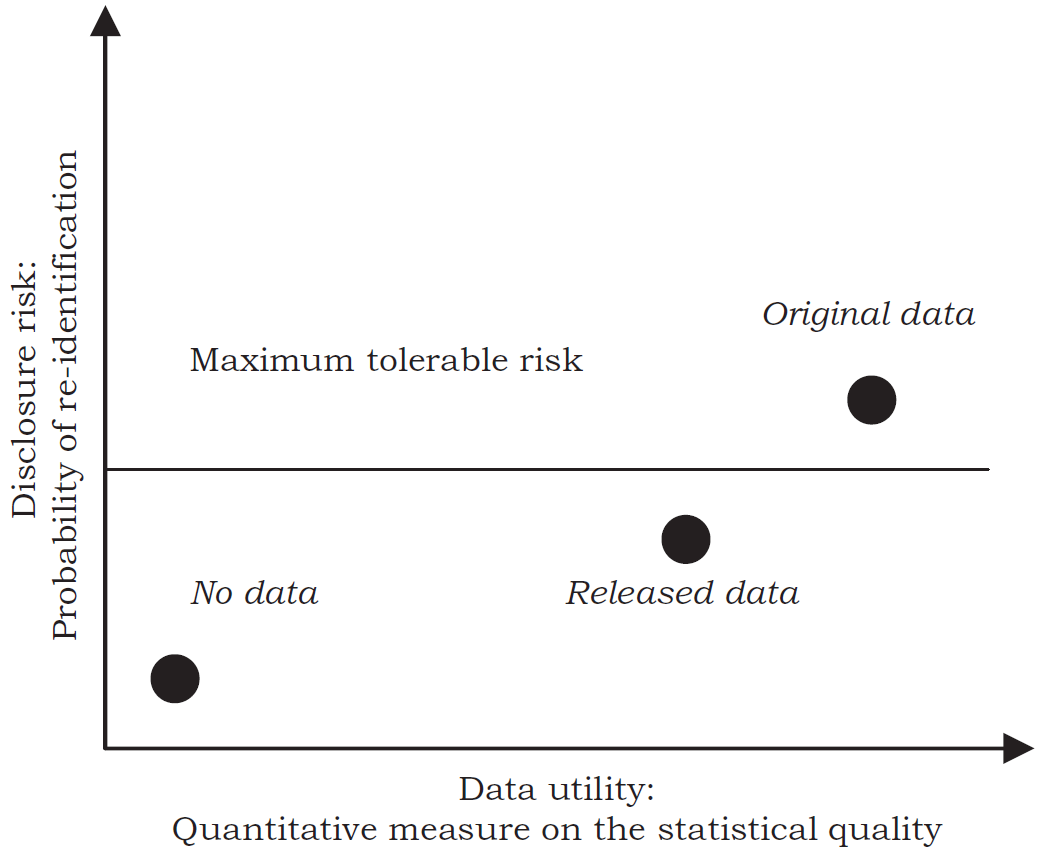
\includegraphics[width=0.5\textwidth,height=\textheight]{gallery/R-U confidentiality map.png}

}

\caption{R-U confidentiality map (Duncan et al.,2001)}

\end{figure}
\end{frame}

\begin{frame}{Disclosure risk}
\protect\hypertarget{disclosure-risk}{}
A unit is at risk of disclosure when it cannot be confused with several
other units
\end{frame}

\begin{frame}{Re-identification risk}
\protect\hypertarget{re-identification-risk}{}
\begin{itemize}
\item
  \color{red}{attacker scenarios and risk measures in more detail using examples}
\end{itemize}
\end{frame}

\begin{frame}{k-anonymity}
\protect\hypertarget{k-anonymity}{}
A data set is said to satisfy k-anonymity for k \textgreater{} 1 if, for
each combination of values of quasi-identifiers (e.g.~name, address,
age, gender, etc.), at least k records exist in the data set sharing
that combination.
\end{frame}

\begin{frame}{Variables}
\protect\hypertarget{variables}{}
\begin{enumerate}
\tightlist
\item
  Identifiers
\item
  Quasi-identifiers or key variables
\item
  Confidential outcome variables
\item
  Non-confidential outcome variables
\end{enumerate}
\end{frame}

\begin{frame}{Disclosure control methods}
\protect\hypertarget{disclosure-control-methods}{}
\begin{enumerate}
\tightlist
\item
  Masking original data

  \begin{enumerate}
  [i.]
  \tightlist
  \item
    Non-perturbative masking.
  \item
    Perturbative masking.
  \end{enumerate}
\item
  Generating synthetic data
\end{enumerate}
\end{frame}

\begin{frame}{Packages for SDC - Microdata (Unit-level data)}
\protect\hypertarget{packages-for-sdc---microdata-unit-level-data}{}
\href{https://cran.r-project.org/web/packages/sdcMicro/index.html}{\color{blue}\underline{\textbf{sdcMicro}}}
can be used to anonymize data, i.e.~to create anonymized files for
public and scientific use. It implements a wide range of methods for
anonymizing categorical and continuous (key) variables. The package also
contains a graphical user interface, which is available by calling the
function sdcGUI.

\href{https://cran.r-project.org/web/packages/simPop/index.html}{\color{blue}\underline{\textbf{simPop}}}
using linear and robust regression methods, random forests (and many
more methods) to simulate synthetic data from given complex data. It is
also suitable to produce synthetic data when the data have hierarchical
and cluster information (such as persons in households) as well as when
the data had been collected with a complex sampling design. It makes use
of parallel computing internally.

\href{https://cran.r-project.org/web/packages/synthpop/index.html}{\color{blue}\underline{\textbf{synthpop}}}
using regression tree methods to simulate synthetic data from given
data. It~is suitable to produce synthetic data when the data have no
hierarchical and cluster information (such as households) as well as
when the data does not collected with a~complex sampling design.
\end{frame}

\begin{frame}{Packages for SDC - Tabular data (Aggregated data)}
\protect\hypertarget{packages-for-sdc---tabular-data-aggregated-data}{}
\href{https://cran.r-project.org/web/packages/sdcTable/index.html}{\color{blue}\underline{\textbf{sdcTable}}}
can be used to provide confidential (hierarchical) tabular data. It
includes the HITAS and the HYPERCUBE technique and uses linear
programming packages (Rglpk and lpSolveAPI) for solving (a large amount
of) linear programs.

\href{https://cran.r-project.org/web/packages/sdcSpatial/index.html}{\color{blue}\underline{\textbf{sdcSpatial}}}
can be used to smooth or/and suppress raster cells in a map. This is
useful when plotting raster-based counts on a map. sdcHierarchies
provides methods to generate, modify, import and convert nested
hierarchies that are often used when defining inputs for statistical
disclosure control methods.

\href{https://cran.r-project.org/web/packages/SmallCountRounding/index.html}{\color{blue}\underline{\textbf{SmallCountRounding}}}
can be used to protect frequency tables by rounding necessary inner
cells so that cross-classifications to be published are safe.

\href{https://cran.r-project.org/web/packages/GaussSuppression/index.html}{\color{blue}\underline{\textbf{GaussSuppression}}}
can be used to protect tables by suppression using the Gaussian
elimination secondary suppression algorithm.
\end{frame}

\begin{frame}{Non-perturbation methods}
\protect\hypertarget{non-perturbation-methods}{}
Non-perturbative masking does not rely on distortion of the original
data but on partial suppressions or reductions of detail.

\begin{longtable}[]{@{}lcc@{}}
\caption{Non-perturbative methods vs.~data types.}\tabularnewline
\toprule\noalign{}
Method & Continuous data & Categorical data \\
\midrule\noalign{}
\endfirsthead
\toprule\noalign{}
Method & Continuous data & Categorical data \\
\midrule\noalign{}
\endhead
Sampling & & X \\
Global recoding & X & X \\
Top and bottom coding & X & X \\
Local suppression & & X \\
\bottomrule\noalign{}
\end{longtable}
\end{frame}

\begin{frame}{sdcMicro}
\protect\hypertarget{sdcmicro}{}
\begin{itemize}
\item
  sdcMicro is an R package for statistical disclosure control.
\item
  \url{https://cran.r-project.org/web/packages/sdcMicro/index.html}
\item
  \url{https://github.com/sdcTools/sdcMicro}
\end{itemize}
\end{frame}

\begin{frame}{sdcMicro}
\protect\hypertarget{sdcmicro-1}{}
\begin{figure}

{\centering 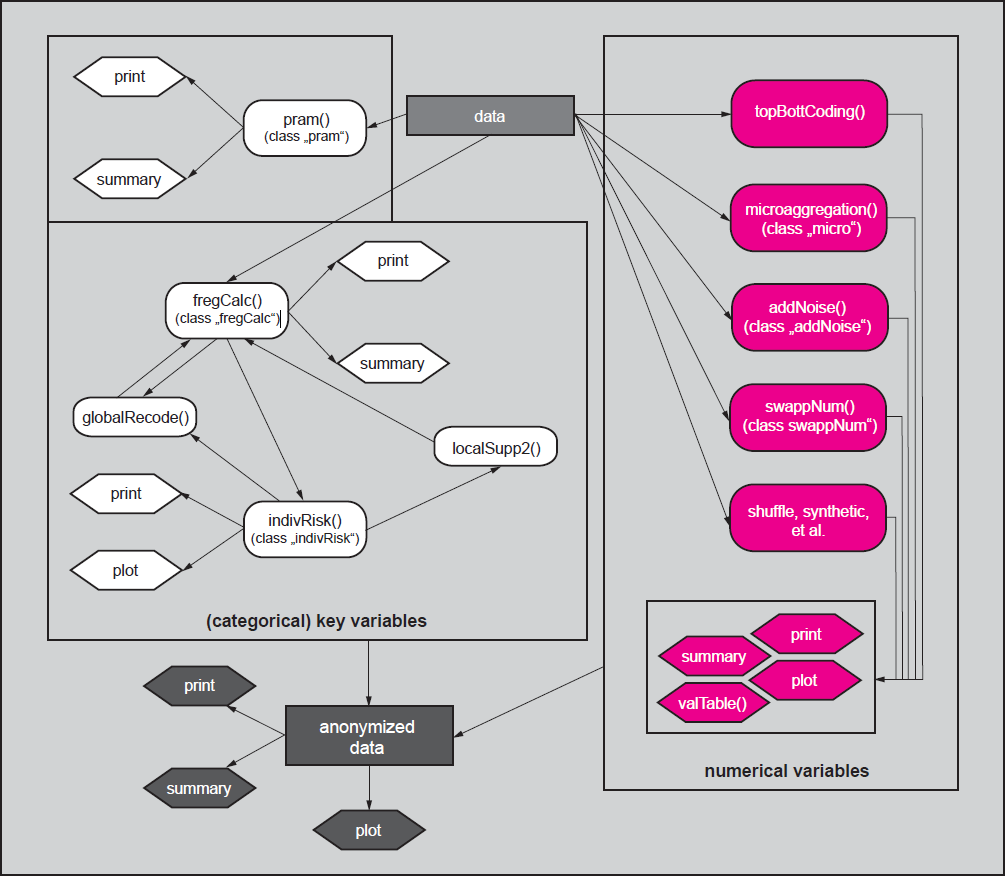
\includegraphics[width=0.55\textwidth,height=\textheight]{gallery/sdcMicro.png}

}

\caption{Certain procedures in package \emph{sdcMicro} and their
relationship}

\end{figure}
\end{frame}

\begin{frame}{Perturbation methods}
\protect\hypertarget{perturbation-methods}{}
\begin{itemize}
\item
  \begin{itemize}
  \item
    \color{red}{sdcMicro}
  \end{itemize}
\end{itemize}
\end{frame}

\begin{frame}{Synthetic methods}
\protect\hypertarget{synthetic-methods}{}
\begin{itemize}
\item
  \color{red}{Introduction to synthetic data}
\item
  \Huge \color{red}{for Jiri/Oscar}
\end{itemize}
\end{frame}

\begin{frame}{Synthetic methods: synthpop}
\protect\hypertarget{synthetic-methods-synthpop}{}
\begin{itemize}
\item
  \color{red}{Generating synthetic data with synthpop}
\item
  \Huge \color{red}{for Jiri/Oscar}
\end{itemize}
\end{frame}

\begin{frame}{Synthetic methods: simPop}
\protect\hypertarget{synthetic-methods-simpop}{}
\begin{itemize}
\item
  \color{red}{Generating synthetic data with simPop}
\item
  \Huge \color{red}{for Jiri/Oscar}
\end{itemize}
\end{frame}

\begin{frame}{Synthetic methods: GANS}
\protect\hypertarget{synthetic-methods-gans}{}
\begin{itemize}
\item
  \color{red}{Generating synthetic data with GANs}
\item
  \Huge \color{red}{for Marco}
\end{itemize}
\end{frame}

\begin{frame}{}
\protect\hypertarget{section}{}
\centering

\Huge Thank you for your attention\\


\includegraphics[width=0.8\textwidth,height=\textheight]{gallery/SwissAnon.png}

\large Swiss Data Anonymization Competence Center

\href{https://swissanon.ch}{\color{blue}\underline{https://swissanon.ch}}
\end{frame}



\end{document}
